\chapter{Cadre Général du Projet}
\label{chap:cadre-general}
\vspace{1em}
\noindent\textbf{\large Sommaire}
\vspace{0.5em}
\localtableofcontents
\clearpage

Ce chapitre pose le cadre général dans lequel s'inscrit le présent projet. Il présente d'abord l'organisme d'accueil, la Banque de Tunisie et des Émirats (BTE), et son contexte de transformation numérique, avant d'introduire le concept du KYC et ses évolutions réglementaires. L'analyse critique des pratiques internes et des solutions commerciales disponibles permet ensuite de formuler la problématique centrale du projet et d'en déduire la solution proposée. Le chapitre se conclut par la présentation de la méthodologie hybride retenue, qui structure l'ensemble du développement.


%=============================================================
\section{Organisme d'accueil}
\label{sec:organisme-accueil}
%=============================================================

Cette section présente l'organisme d'accueil du projet, la Banque de Tunisie et des Émirats, ainsi que sa structure organisationnelle, afin de situer le contexte institutionnel dans lequel s'inscrit le développement de la solution eKYC.

\subsection{Présentation de la BTE}
\label{subsec:presentation-bte}

La Banque de Tunisie et des Émirats (BTE), dont le logo est présenté en Figure~\ref{fig:ch1-logo-bte}, est un établissement bancaire tunisien fondé en 1982 dans le cadre d'un partenariat entre l'Abou Dhabi Investment Authority (ADIA) et le gouvernement tunisien. Au c\oe{}ur de sa gouvernance opérationnelle, la Direction Centrale de l'Informatique et de l'Organisation (DCIO) pilote la stratégie de transformation numérique de l'établissement, en coordonnant les initiatives technologiques à l'échelle de l'ensemble des directions métiers. L'expression la plus concrète de cette dynamique est le lancement de \og NEO BTE \fg{} : une plateforme bancaire en ligne (web, iOS, Android) intégrant un parcours d'ouverture de compte avec numérisation des documents d'identité, constituant ainsi le point de départ direct du présent projet.
\begin{figure}[H]
  \centering
  
\includegraphics[width=0.45\textwidth]{images/image_ch1/logo_bte.png}
  \caption{\textit{Logo officiel de la Banque de Tunisie et des Émirats (BTE)}}
  \label{fig:ch1-logo-bte}
\end{figure}
\subsection{Organigramme de la BTE}
\label{subsec:organigramme-bte}

La Figure~\ref{fig:ch1-organigramme} montre l'organisation de la BTE. La Direction Centrale de l'Informatique et de l'Organisation (DCIO) regroupe trois directions : la Direction Informatique, la Direction Système et Sécurité Fonctionnelle, et la Direction de l'Organisation. La Direction Informatique est composée de deux départements : le Département Développement, chargé de la création et de l'amélioration des applications, et le Département Support Informatique, qui assure l'assistance technique aux utilisateurs.

\begin{figure}[H]
  \centering
  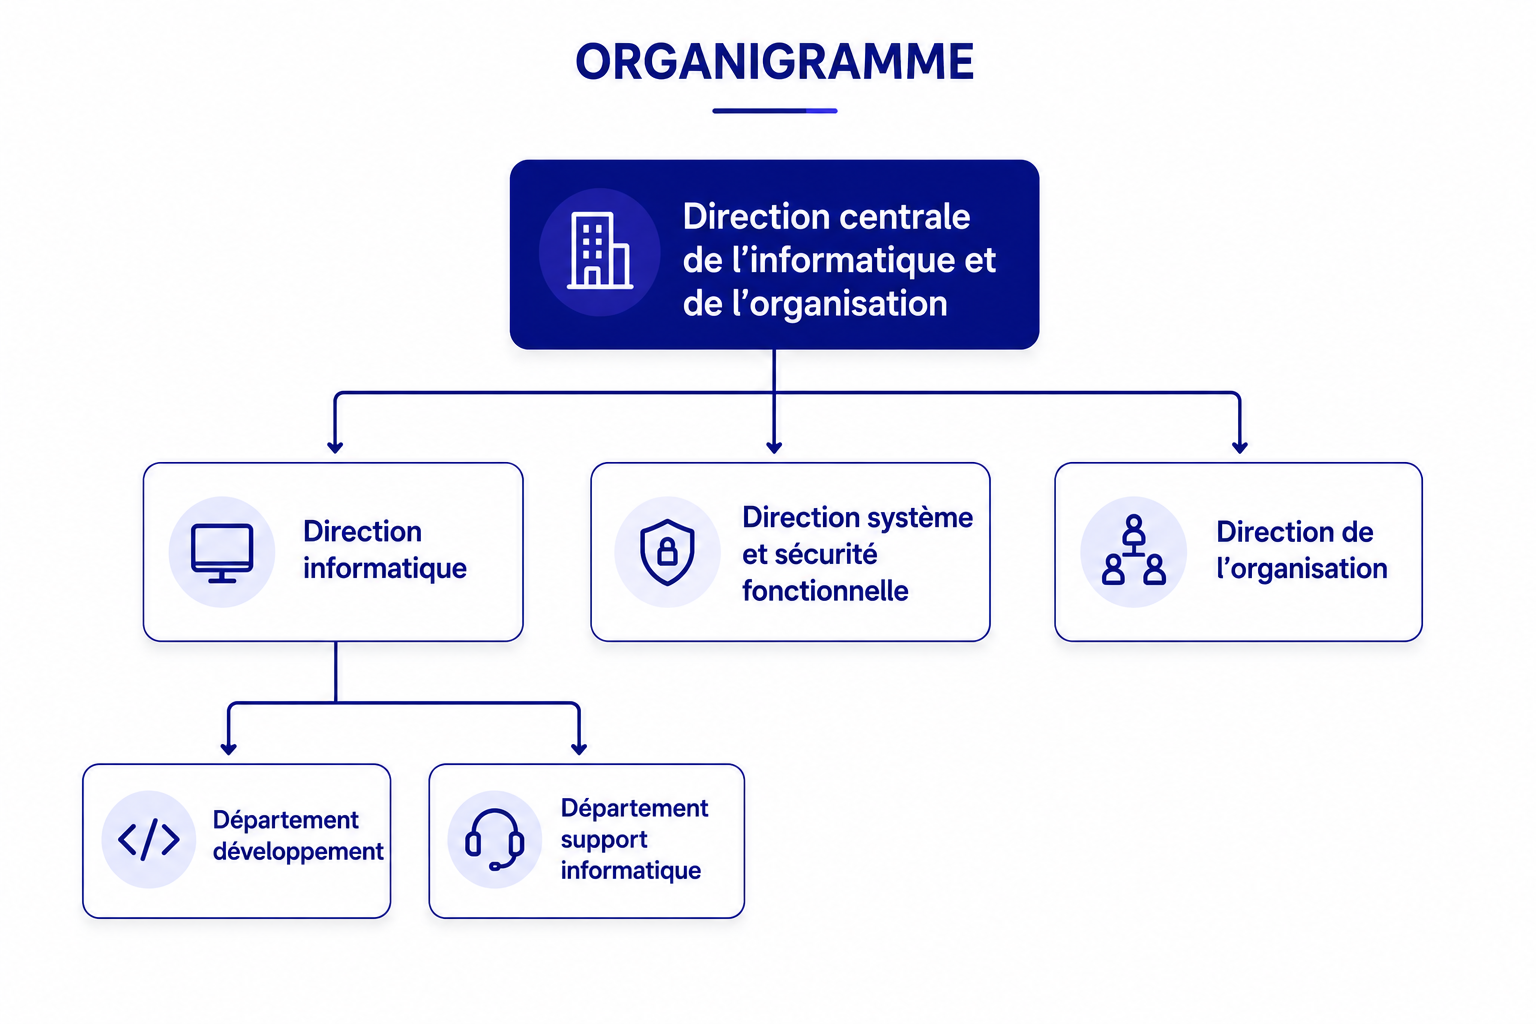
\includegraphics[width=0.75\textwidth]{images copy/image_ch1/organigramme.png}
  \caption{\textit{Organigramme de la Banque de Tunisie et des Émirats}}
  \label{fig:ch1-organigramme}
\end{figure}

Ancrée dans cette dynamique de digitalisation, la BTE fait face à un enjeu réglementaire et opérationnel central : la modernisation de son processus de vérification d'identité client, communément désigné sous le terme KYC.


%=============================================================
\section{Compréhension du métier KYC}
\label{sec:comprehension-kyc}
%=============================================================

Dans un secteur bancaire soumis à des exigences réglementaires croissantes, la maîtrise de l'identité client est devenue un impératif non négociable. Le KYC (\textit{Know Your Customer}), ou \og Connaissance du Client \fg{}, désigne l'ensemble des procédures permettant à un établissement financier d'authentifier ses clients et de se conformer aux normes de lutte contre le blanchiment d'argent et le financement du terrorisme (LCB-FT). Cette section examine d'abord les deux formes que prend ce processus --- traditionnel et automatisé --- avant de présenter le cadre réglementaire qui l'encadre.

\subsection{KYC traditionnel vs KYC automatisé}
\label{subsec:kyc-traditionnel-vs-automatise}

Cette sous-section confronte le modèle KYC traditionnel, entièrement manuel, à son évolution automatisée, afin de mettre en lumière les apports du e-KYC et de justifier l'orientation technologique du présent projet.

\subsubsection{Le KYC traditionnel}

Historiquement, le processus KYC repose sur des interactions physiques ou semi-numériques. Le client soumet des documents d'identité (Carte Nationale d'Identité, Passeport) qui sont ensuite contrôlés par des agents humains, selon deux modalités distinctes.

\paragraph{Processus hors ligne}
Dans ce mode, le client se déplace en agence pour remettre ses documents en main propre. L'agent de back-office procède à une vérification manuelle, saisit les données dans le système d'information et notifie le client de l'issue du contrôle. Ce processus séquentiel est visualisé à travers la Figure~\ref{fig:ch1-kyc-hors-ligne}.

\begin{figure}[H]
  \centering
  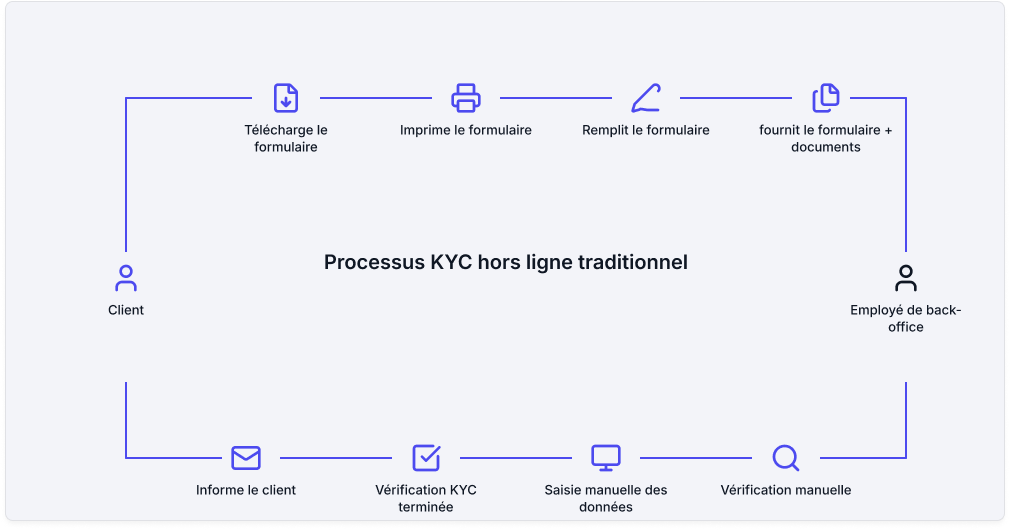
\includegraphics[width=0.75\textwidth]{images/image_ch1/SLIDE 1_ Hors ligne3.png}
  \caption{\textit{Processus KYC traditionnel hors ligne}}
  \label{fig:ch1-kyc-hors-ligne}
\end{figure}

\paragraph{Processus en ligne}
La variante en ligne, illustrée par la Figure~\ref{fig:ch1-kyc-en-ligne}, permet au client de soumettre ses documents via le portail numérique de l'établissement. Malgré la dématérialisation du canal, la vérification reste entièrement manuelle : un opérateur examine chaque pièce transmise avant de valider ou de rejeter le dossier.

\begin{figure}[H]
  \centering
  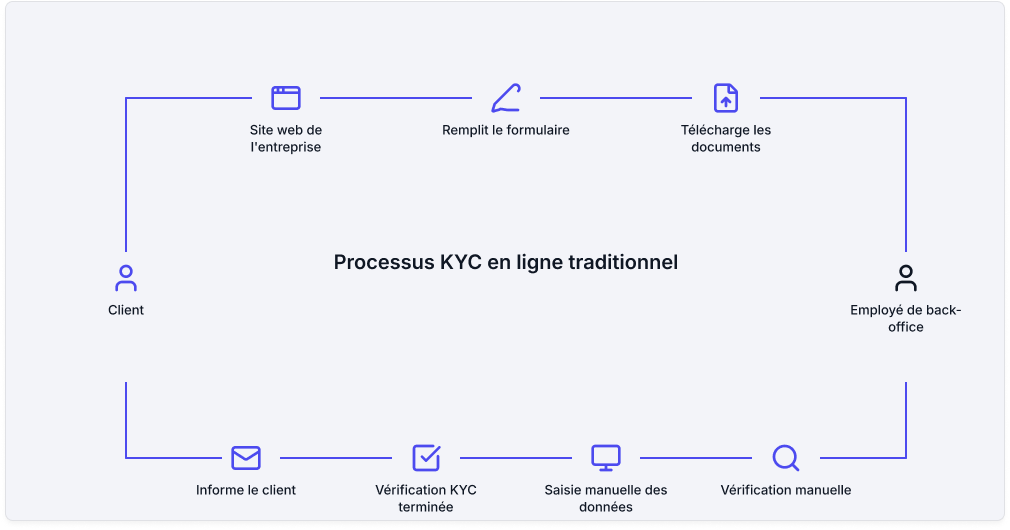
\includegraphics[width=0.75\textwidth]{images/image_ch1/SLIDE 2_ En ligne.png}
  \caption{\textit{Processus KYC traditionnel en ligne}}
  \label{fig:ch1-kyc-en-ligne}
\end{figure}

\paragraph{Limites structurelles du KYC traditionnel}
Qu'il soit réalisé en agence ou via un portail numérique, le KYC traditionnel présente des failles communes qui fragilisent son aptitude à répondre aux exigences croissantes des institutions financières modernes : des délais de traitement significatifs qui dégradent l'expérience client, un risque d'erreurs humaines lors de la saisie ou de la vérification manuelle pouvant induire des faux positifs ou des failles de conformité, et une mobilisation importante de ressources humaines difficiles à faire évoluer face à la croissance du portefeuille clients.

\subsubsection{Le KYC automatisé (e-KYC)}

Sous l'impulsion de la transformation digitale, les institutions financières migrent progressivement vers des solutions de e-KYC (\textit{Electronic KYC}). Cette approche substitue l'intervention humaine par des traitements algorithmiques intelligents, capables d'analyser, d'extraire et de valider les informations d'identité en temps réel. Ce nouveau paradigme repose sur un enchaînement fluide d'étapes entièrement automatisées, comme le montre la Figure~\ref{fig:ch1-kyc-automatise}.

\begin{figure}[H]
  \centering
  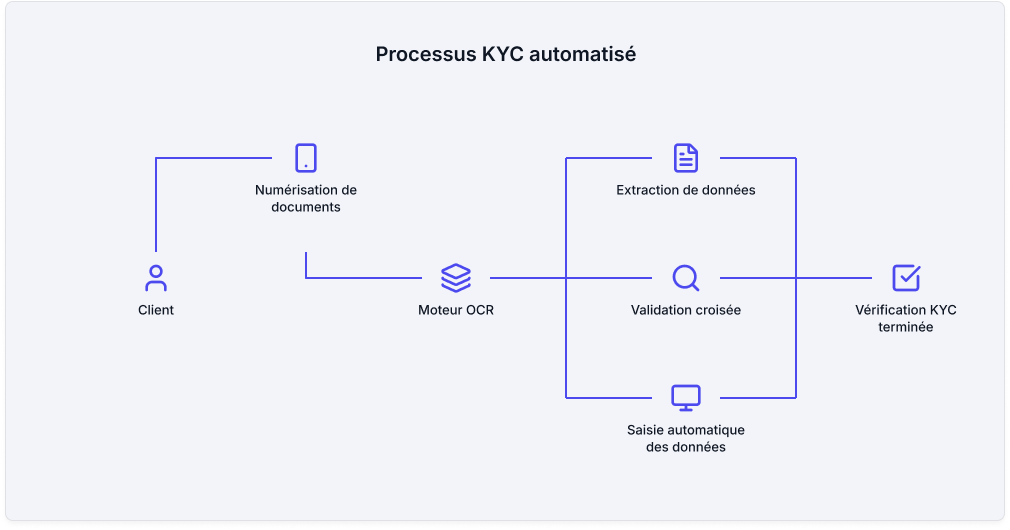
\includegraphics[width=0.75\textwidth]{images/image_ch1/SLIDE 3_ Automatis.png}
  \caption{\textit{Processus KYC automatisé}}
  \label{fig:ch1-kyc-automatise}
\end{figure}

Le workflow du e-KYC, tel qu'illustré par la figure ci-dessus, se déroule en quatre étapes enchaînées automatiquement :

\begin{enumerate}
  \item Numérisation des documents d'identité via smartphone ou scanner.
  \item Traitement par un moteur OCR pour l'extraction des données textuelles.
  \item Validation croisée et saisie automatique des données extraites dans le système.
  \item Vérification KYC complète, sans intervention humaine.
\end{enumerate}

Cette automatisation offre des avantages stratégiques concrets : un traitement quasi instantané contre plusieurs heures en mode manuel, une réduction des coûts back-office, une détection algorithmique et reproductible des fraudes documentaires, et un parcours 100\,\% digital disponible 24h/24 depuis n'importe quel appareil.

\subsection{Cadre réglementaire et normatif}
\label{subsec:cadre-reglementaire}

Toute solution de KYC automatisé doit s'inscrire dans un cadre légal rigoureux. Cette sous-section présente les normes internationales et les réglementations nationales tunisiennes qui encadrent le déploiement de la solution eKYC de la BTE.

\subsubsection{Normes internationales}

Déployer un système eKYC dans un environnement bancaire réglementé implique de respecter des standards internationaux qui définissent les obligations minimales en matière de vigilance client. Le Tableau~\ref{tab:normes-intl} présente les deux références les plus déterminantes pour le périmètre de ce projet.

\begin{longtable}{|p{3.8cm}|p{6cm}|p{4cm}|}
  \toprule
  \rowcolor{bleu_principal}
  \textcolor{white}{\textbf{Référence}} & \textcolor{white}{\textbf{Description}} & \textcolor{white}{\textbf{Source}} \\
  \midrule
  \endfirsthead
  \toprule
  \rowcolor{bleu_principal}
  \textcolor{white}{\textbf{Référence}} & \textcolor{white}{\textbf{Description}} & \textcolor{white}{\textbf{Source}} \\
  \midrule
  \endhead
  Groupe d'Action Financière (GAFI) --- Recommandation 10 &
  Organisme international fixant les standards mondiaux LCB-FT, notamment la vigilance client (\textit{Customer Due Diligence}). &
  {\scriptsize\textcolor{bleu_clair}{\url{https://www.fatf-gafi.org}}} \newline {\scriptsize\textit{Consulté le 18/03/2026}} \\
  \midrule
  Règlement Général sur la Protection des Données (RGPD) &
  Applicable aux solutions traitant des données de ressortissants ou de filiales de banques européennes. Exige la sécurisation des données biométriques et personnelles. &
  \begin{minipage}[t]{4cm}{\scriptsize\textit{Règlement (UE) 2016/679 du Parlement européen}}\newline{\scriptsize\textit{Consulté le 18/03/2026}}\end{minipage} \\
  \bottomrule
  \caption{Normes réglementaires internationales}
  \label{tab:normes-intl}
\end{longtable}

\subsubsection{Réglementations nationales (Tunisie)}

Au plan national, la solution eKYC de la BTE doit se conformer à un corpus législatif tunisien qui encadre à la fois l'identification des clients, le contrôle interne et la protection des données personnelles. Le Tableau~\ref{tab:normes-natl} en synthétise les textes fondateurs.

\begin{longtable}{|p{4cm}|p{5.5cm}|p{4cm}|}
  \toprule
  \rowcolor{bleu_principal}
  \textcolor{white}{\textbf{Référence}} & \textcolor{white}{\textbf{Description}} & \textcolor{white}{\textbf{Source}} \\
  \midrule
  \endfirsthead
  \toprule
  \rowcolor{bleu_principal}
  \textcolor{white}{\textbf{Référence}} & \textcolor{white}{\textbf{Description}} & \textcolor{white}{\textbf{Source}} \\
  \midrule
  \endhead
  Loi organique n°~2015-26 (modifiée par la loi n°~2019-9) &
  Texte fondateur imposant aux banques tunisiennes l'identification rigoureuse de leurs clients, en conformité avec les recommandations du GAFI. &
  {\scriptsize\textcolor{bleu_clair}{\href{https://www.ohchr.org/sites/default/files/lib-docs/HRBodies/UPR/Documents/Session27/TN/26Annexe16Loi2015_26fr.pdf}{ohchr.org --- Loi 2015-26}}}\newline{\scriptsize\textit{Consulté le 18/03/2026}} \\
  \midrule
  Circulaire de la Banque Centrale de Tunisie (BCT) n°~2018-09~\cite{bct2018circulaire} &
  Fixe les règles de contrôle interne et de conformité, obligeant les établissements à déployer des procédures de vigilance \textit{Know Your Customer}. &
  {\scriptsize\textcolor{bleu_clair}{\url{https://www.bct.gov.tn/bct/siteprod/documents/Cir_2025_06_fr.pdf}}} \newline {\scriptsize\textit{Consulté le 18/03/2026}} \\
  \midrule
  Loi organique n°~2004-63 --- Instance Nationale de Protection des Données Personnelles (INPDP) &
  Toute solution KYC collectant des images de CIN en Tunisie doit être déclarée à l'INPDP. Notre solution y répond via un traitement local, selon les principes de \textit{Privacy by Design}. &
  {\scriptsize\textcolor{bleu_clair}{\url{https://www.inpdp.tn/ressources/loi_2004.pdf}}} \newline {\scriptsize\textit{Consulté le 18/03/2026}} \\
  \midrule
  Commission Tunisienne des Analyses Financières (CTAF) / Banque Centrale de Tunisie (BCT) / Conseil du Marché Financier (CMF) &
  Principaux régulateurs supervisant respectivement la conformité LCB-FT et les rapports de transactions suspectes, les institutions financières, et les marchés de capitaux. &
  \begin{minipage}[t]{3.8cm}
    {\scriptsize\textcolor{bleu_clair}{\url{https://www.ctaf.gov.tn}}}\newline
    {\scriptsize\textcolor{bleu_clair}{\url{https://www.bct.gov.tn}}}\newline
    {\scriptsize\textcolor{bleu_clair}{\url{https://www.cmf.tn}}}\newline
    {\scriptsize\textit{Consultés le 18/03/2026}}
  \end{minipage} \\
  \bottomrule
  \caption{Réglementations nationales tunisiennes}
  \label{tab:normes-natl}
\end{longtable}

Le passage du KYC traditionnel vers le e-KYC représente une rupture profonde dans la gestion de l'identité client : en substituant les traitements manuels par des pipelines intelligents (OCR, vision par ordinateur, intelligence artificielle) les établissements financiers gagnent en rapidité, en précision et en conformité. Encadrée par un corpus réglementaire solide, cette évolution s'impose désormais comme un levier stratégique incontournable pour toute institution souhaitant conjuguer efficacité opérationnelle et robustesse réglementaire.


%=============================================================
\section{Position du problème}
\label{sec:position-probleme}
%=============================================================

Cette section analyse l'existant à deux niveaux : d'abord le processus KYC interne de la BTE et ses faiblesses, puis les solutions commerciales disponibles sur le marché et leurs limites dans le contexte spécifique de la banque. Cette double analyse conduit à formuler la problématique centrale du projet.

\subsection{KYC interne de la BTE et analyse critique}
\label{subsec:etude-existant}

Cette sous-section examine le fonctionnement actuel du processus KYC au sein de la BTE, puis en dresse un bilan critique pour identifier les failles structurelles qui justifient l'automatisation.

\subsubsection{KYC au sein de la BTE}

Au sein de la BTE, le processus KYC s'articule autour de deux modes complémentaires : un traitement réalisé en agence et un parcours digital accessible via l'application mobile NEO BTE. Ces deux modes, dont le fonctionnement détaillé a été présenté en section~\ref{subsec:kyc-traditionnel-vs-automatise}, sont ici examinés sous l'angle de leur mise en œuvre concrète au sein de l'établissement. Si ces deux canaux couvrent des usages distincts, ils partagent une caractéristique fondamentale : tous deux reposent entièrement sur une vérification manuelle par des agents humains, sans aucune automatisation du traitement documentaire. La Figure~\ref{fig:ch1-kyc-modes} met en regard ces deux modalités et souligne leur dénominateur commun : la dépendance à l'intervention humaine.

\begin{figure}[H]
  \centering
  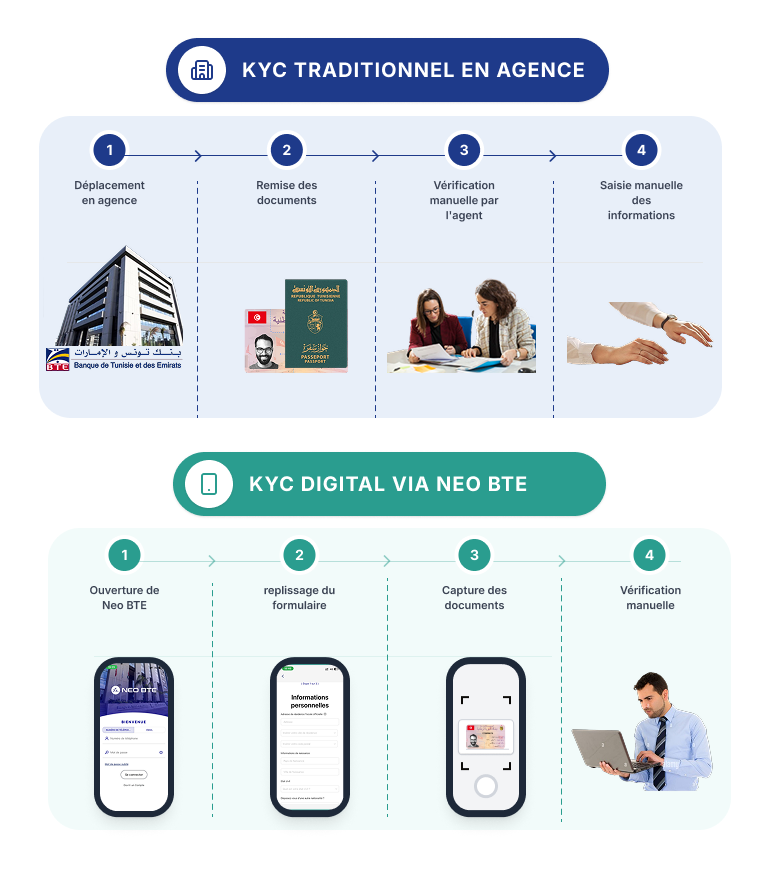
\includegraphics[width=0.75\textwidth]{images/image_ch1/KYC_Agence_Vs_NeoBte.png}
  \caption{\textit{KYC Traditionnel en agence vs Digital via NEO BTE}}
  \label{fig:ch1-kyc-modes}
\end{figure}

\subsubsection{Analyse critique du processus interne}

L'examen du processus KYC interne met en évidence quatre failles structurelles majeures.

\begin{itemize}
  \item \textbf{Délais incompatibles avec le digital :} la vérification manuelle impose des temps de traitement qui dégradent l'expérience d'onboarding et contrastent avec les attentes d'un client NEO BTE habitué à l'instantané.
  \item \textbf{Faillibilité humaine :} les erreurs de saisie et d'appréciation visuelle sont inévitables à grande échelle, pouvant générer des faux positifs ou des omissions de conformité engageant la responsabilité de la banque vis-à-vis de la BCT.
  \item \textbf{Vulnérabilité à la fraude documentaire :} face à des documents retouchés ou des identités usurpées, l'œil humain ne peut garantir une détection systématique et reproductible.
  \item \textbf{Difficulté de passage à l'échelle :} le modèle manuel ne peut absorber la croissance du portefeuille clients NEO BTE sans une augmentation proportionnelle des effectifs, rendant le système structurellement non scalable.
\end{itemize}

\subsection{Solutions KYC commerciales et leurs limites}
\label{subsec:solutions-commerciales}

Face aux faiblesses du processus interne, trois plateformes représentatives du marché ont été étudiées pour évaluer leur pertinence dans le contexte spécifique de la BTE. Chacune a été analysée selon des critères déterminants (couverture fonctionnelle, support du contexte tunisien, dépendance cloud et personnalisabilité ).

\subsubsection{Présentation des solutions étudiées}

Trois plateformes ont été analysées selon des critères déterminants pour le contexte de la BTE.

\paragraph{uqudo~\cite{uqudo2026}}
Plateforme complète intégrant OCR, biométrie et détection de fraude, accessible via une API cloud avec support multilingue. Elle couvre un périmètre fonctionnel large mais repose entièrement sur une infrastructure externe.

\paragraph{NEUROPARSER~\cite{neuroparser2026}}
Solution spécialisée dans l'OCR de la carte d'identité nationale tunisienne. Bien qu'elle offre un support natif de la CIN, son périmètre se limite à l'extraction de données textuelles, sans capacités biométriques ni détection d'anomalies.

\paragraph{FACEKI~\cite{faceki2026}}
Solution orientée vers la vérification biométrique et l'analyse documentaire, offrant des garanties de sécurité avancées, mais dépendant entièrement d'une infrastructure cloud externe.

Le Tableau~\ref{tab:solutions-kyc} synthétise cette analyse comparative selon les critères les plus déterminants pour le contexte de la BTE.

\begin{table}[H]
  \centering
  \small
  \begin{tabular}{|l|c|c|c|}
    \toprule
    \rowcolor{bleu_principal}
    \textcolor{white}{\textbf{Critère}} & \textcolor{white}{\textbf{uqudo}} & \textcolor{white}{\textbf{NEUROPARSER}} & \textcolor{white}{\textbf{FACEKI}} \\
    \midrule
    Périmètre fonctionnel & AML + Biométrie & OCR uniquement & Biométrie + Docs \\
    \midrule
    \rowcolor{gris_leger}
    Support CIN tunisienne & Partiel & \textbf{OUI} & Partiel \\
    \midrule
    Détection de fraude & \textbf{OUI} & NON & \textbf{OUI} \\
    \midrule
    \rowcolor{gris_leger}
    Intégration API & \textbf{OUI} & \textbf{OUI} & \textbf{OUI} \\
    \midrule
    Sensibilité qualité image & Modérée & Élevée & Modérée \\
    \midrule
    \rowcolor{gris_leger}
    Dépendance cloud & Forte & Forte & Forte \\
    \midrule
    Coût & Élevé & Modéré & Élevé \\
    \midrule
    \rowcolor{gris_leger}
    Personnalisation & Limitée & Limitée & Limitée \\
    \bottomrule
  \end{tabular}
  \caption{Comparaison des solutions KYC commerciales : uqudo, NEUROPARSER et FACEKI}
  \label{tab:solutions-kyc}
\end{table}

\subsubsection{Limites par rapport au contexte de la BTE}

L'analyse comparative révèle que les trois solutions partagent des limites rédhibitoires pour la BTE.

\begin{itemize}
  \item \textbf{Dépendance cloud systématique :} les trois plateformes analysées transmettent les données documentaires vers des serveurs externes, soulevant des enjeux de souveraineté des données incompatibles avec les exigences d'un établissement bancaire réglementé.
  \item \textbf{Inadaptation au contexte tunisien :} le traitement bilingue arabe/latin, propre à la CIN et au passeport tunisiens, n'est que partiellement ou non pris en charge, dégradant la fiabilité de l'extraction.
  \item \textbf{Coûts, rigidité et dépendance stratégique :} les licences propriétaires sont élevées, les modèles ne sont pas personnalisables et aucune adaptation aux évolutions des documents nationaux ou aux exigences de la BCT n'est possible, privant la BTE de toute autonomie sur l'évolution de son système.
  \item \textbf{Sensibilité aux conditions de capture mobile :} la qualité variable des images prises en situation réelle entraîne des taux d'échec significatifs, non compensés par des mécanismes de robustesse intégrés.
\end{itemize}

Ces constats convergent vers une conclusion sans appel : ni le processus interne actuel, ni les solutions propriétaires disponibles ne sont en mesure de répondre aux ambitions portées par la stratégie NEO BTE.

\subsection{Problématique }
\label{subsec:problematique}

L'ensemble des faiblesses identifiées converge vers une problématique unique, à la fois opérationnelle et stratégique. Le KYC manuel constitue aujourd'hui un frein structurel à la stratégie digitale de la BTE : il est incapable de répondre à la montée en charge qu'exige la croissance rapide du portefeuille clients NEO BTE, il compromet la fluidité du parcours d'onboarding et alourdit les coûts de traitement, et il fragilise la posture de conformité de l'établissement face aux exigences de la BCT. Parallèlement, les solutions commerciales analysées s'avèrent inadaptées aux contraintes réglementaires, documentaires et de souveraineté des données propres au contexte tunisien. Ce double constat impose de formuler la question centrale suivante :

\begin{quote}
\textit{\textbf{Comment concevoir une solution KYC automatisée, internalisée et adaptée au contexte tunisien, capable d'extraire, de classifier et de valider des documents d'identité avec fiabilité, tout en garantissant la conformité aux directives de la BCT et la souveraineté des données de la BTE ?}}
\end{quote}

Cette problématique engage trois défis techniques majeurs : l'extraction précise de données textuelles sur des documents multilingues et de qualité variable, la robustesse du système face aux conditions réelles de capture mobile, et l'intégration du module IA dans un \textit{workflow} bancaire structuré, modulaire et auditable.

\subsection{Solution proposée}
\label{subsec:solution-proposee}

Le présent projet propose de concevoir un système eKYC développé sur mesure pour la BTE, dont le c\oe{}ur est un pipeline d'intelligence artificielle automatisé. Avant même la soumission du dossier, le système détecte automatiquement le type de document présenté (CIN, passeport). Dès la soumission, il prend en charge sans action manuelle l'extraction des données par reconnaissance optique de caractères (OCR), la vérification de cohérence des informations extraites, et la détection d'anomalies et de tentatives de fraude documentaire. Ce traitement bout-en-bout garantit une réponse quasi instantanée et reproductible, là où l'opérateur humain introduisait latence et variabilité.

Toutefois, tout système d'IA présente des marges d'erreur résiduelles. C'est pourquoi l'intervention humaine est maintenue comme verrou de décision finale : un agent bancaire conserve la validation ultime sur les dossiers signalés ou ambigus. Le rôle de l'IA est d'assister et d'accélérer l'agent, non de le remplacer intégralement. La solution repose sur trois piliers : une architecture \textit{on-premise} garantissant qu'aucune donnée documentaire ne quitte l'infrastructure bancaire, une adaptation native au contexte tunisien avec des modèles entraînés sur des documents bilingues arabe/latin (CIN, passeport), et une stack entièrement open-source assurant une autonomie totale sur l'évolution du système.


%=============================================================
\section{Méthodologie adoptée }
\label{sec:methodologie}
%=============================================================

Ce projet présente une double nature : d'un côté, un travail de recherche appliquée en intelligence artificielle, soumis à l'incertitude expérimentale ; de l'autre, le développement d'une plateforme bancaire fonctionnelle, aux exigences stables et formalisables. Ni les frameworks purement scientifiques, ni les méthodologies classiques de génie logiciel ne permettent, pris isolément, de répondre efficacement à ces deux dimensions. Une approche hybride a donc été retenue, structurée en deux incréments distincts, chacun piloté par le modèle le plus adapté à sa nature propre.

\subsection{Modèle incrémental}
\label{subsec:modele-incremental}

Le modèle incrémental consiste à construire un système par ajouts successifs et fonctionnels, appelés incréments. Cette approche permet de prioriser les composantes les plus critiques dès le départ, de valider indépendamment chaque bloc avant d'aborder le suivant, et de réduire les risques d'intégration en fin de projet. Ce choix est naturellement justifié par la double complexité du projet, qui se décline selon deux composantes de natures fondamentalement différentes : une composante Intelligence Artificielle (vision par ordinateur, OCR, scoring de documents), caractérisée par une forte incertitude expérimentale et une dépendance importante à la qualité des données d'entraînement, et une composante développement logiciel (backend, frontend, workflow bancaire), nécessitant une architecture claire et une intégration progressive des fonctionnalités. Ces deux composantes présentant une faible interdépendance technique, leur structuration en deux incréments distincts s'impose, tout en préservant la cohérence globale du système livré.

\subsection{CRISP-ML(Q)}
\label{subsec:crisp-mlq}

CRISP-ML(Q) est le modèle retenue pour piloter le premier incrément, consacré au développement du pipeline IA. Cette sous-section en présente les fondements et les six phases structurantes.

\subsubsection{CRISP-ML(Q) vs CRISP-DM}

Avant d'aller plus loin, il convient de situer CRISP-ML(Q) par rapport à son prédécesseur. CRISP-DM (\textit{Cross-Industry Standard Process for Data Mining}), publié en 1999, a longtemps constitué la référence méthodologique pour les projets de fouille de données. Cependant, son adoption aux projets de Machine Learning en production révèle plusieurs lacunes : l'absence de phases dédiées au déploiement continu, à la surveillance en production et, surtout, à l'assurance qualité systématique tout au long du cycle de vie du modèle. CRISP-ML(Q) (\textit{Cross-Industry Standard Process for Machine Learning with Quality Assurance}) comble précisément ces lacunes. Proposé en 2020 par Studer \textit{et al.}~\cite{studer2021crispmlq} , le modèle introduit le \og Q \fg{} pour \textit{Quality} comme philosophie transversale : des contrôles qualité formels sont intégrés à chaque phase du processus, et non uniquement lors de l'évaluation finale. Cette dimension qualité renforcée est particulièrement précieuse dans un contexte bancaire où la fiabilité et l'auditabilité des systèmes IA sont des exigences non négociables.

\subsubsection{Les six phases de CRISP-ML(Q)}

Le 1\textsuperscript{er} incrément du projet est entièrement dédié à la conception, à l'entraînement et à la validation du pipeline d'intelligence artificielle, selon le cadre CRISP-ML(Q). La Figure~\ref{fig:ch1-6-phases-crisp-mlq} présente les six phases qui structurent ce cycle.

\begin{figure}[H]
  \centering
  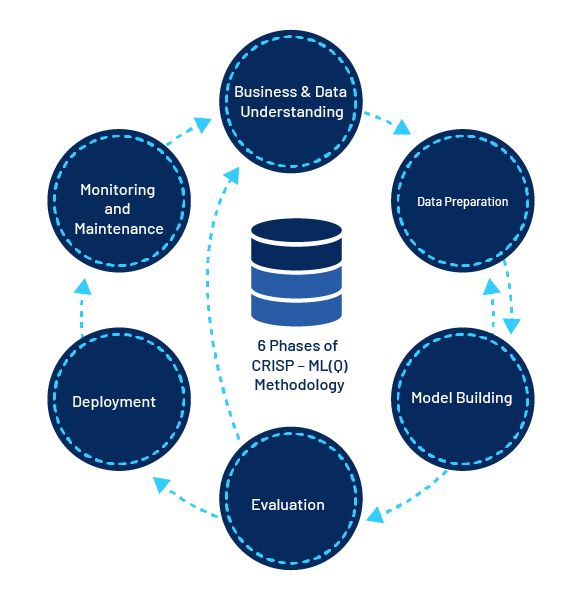
\includegraphics[width=0.75\textwidth]{images/image_ch1/crispMl_Q.png}
  \caption{\textit{Les six phases du modèle CRISP-ML(Q)}}
  \label{fig:ch1-6-phases-crisp-mlq}
\end{figure}

\begin{enumerate}
  \item \textbf{Business \& Data Understanding :} analyse des besoins métiers, identification des types de documents à traiter (CIN, passeport), ainsi que constitution et caractérisation du jeu de données. Un contrôle qualité initial vérifie la représentativité et la pertinence des données collectées.
  \item \textbf{Data Preparation :} nettoyage, transformation, organisation et préparation des données afin de les rendre exploitables pour l'apprentissage. Des métriques qualité sont appliquées pour valider chaque transformation opérée sur le corpus documentaire.
  \item \textbf{Modeling :} entraînement et optimisation des modèles de Deep Learning répondant au problème identifié. Les expériences sont tracées et comparées selon des critères de qualité prédéfinis, garantissant la reproductibilité des résultats.
  \item \textbf{Evaluation \& Quality Assurance :} mesure des performances du modèle et vérification de son adéquation avec les objectifs métier fixés. Cette phase constitue le verrou qualité central avant tout passage en production.
  \item \textbf{Deployment \& Integration :} intégration du modèle validé dans l'architecture applicative. Des tests de non-régression et des vérifications de conformité réglementaire accompagnent cette mise en production.
  \item \textbf{Monitoring \& Maintenance :} suivi continu du modèle déployé, détection des dérives de performance (\textit{data drift}) et maintenance évolutive face aux évolutions des documents et des conditions de capture.
\end{enumerate}

À l'issue de cet incrément, le résultat attendu est un moteur IA opérationnel, capable de détecter les documents soumis, d'en extraire les informations structurées et de fonctionner de manière fiable en conditions réelles, avec des garanties qualité documentées à chaque étape.

\subsection{Modèle en cascade}
\label{subsec:modele-cascade}

Une fois le c{\oe}ur IA validé, le second incrément se consacre au développement de la plateforme applicative dans son intégralité. Pour cette composante logicielle, dont les exigences fonctionnelles sont clairement définies et stables dès le départ, le modèle en cascade s'impose comme le cadre le plus adapté. Il s'agit d'une approche séquentielle et structurée dans laquelle chaque phase doit être achevée et validée avant que la suivante ne commence, garantissant une traçabilité complète des décisions de conception. Appliqué à l'incrément applicatif, il se décline selon les phases suivantes :

\begin{enumerate}
  \item \textbf{Analyse des besoins :} recueil et formalisation des exigences fonctionnelles et non fonctionnelles du système (interfaces agent et client, workflow KYC, intégration du module IA).
  \item \textbf{Conception :} définition de l'architecture logicielle, des modèles de données et des interfaces utilisateur.
  \item \textbf{Implémentation :} développement du back-office destiné aux agents bancaires (gestion des dossiers, supervision des validations, tableau de bord KYC) et du front-office permettant aux clients de soumettre leurs documents et de suivre l'état de leur dossier en temps réel.
  \item \textbf{Intégration \& Tests :} connexion de la plateforme applicative au pipeline intelligent développé lors de l'incrément 1, tests \textit{end-to-end} et validation du système complet.
  \item \textbf{Déploiement :} livraison du système intégré dans l'environnement bancaire cible.
\end{enumerate}

Ce modèle est particulièrement approprié ici car les spécifications du module applicatif sont suffisamment précises et stables pour éviter les allers-retours coûteux que justifieraient des méthodes itératives. Il offre par ailleurs une visibilité claire sur l'avancement du projet et facilite la communication avec les parties prenantes de la BTE.

\subsection{Planification globale du projet}
\label{subsec:planification}

L'approche incrémentale hybride retenue se traduit concrètement par une planification en deux phases successives et cohérentes. La Figure~\ref{fig:ch1-planning} illustre la répartition temporelle des grandes activités du projet selon les deux incréments et leurs jalons principaux.

\begin{figure}[H]
  \centering
  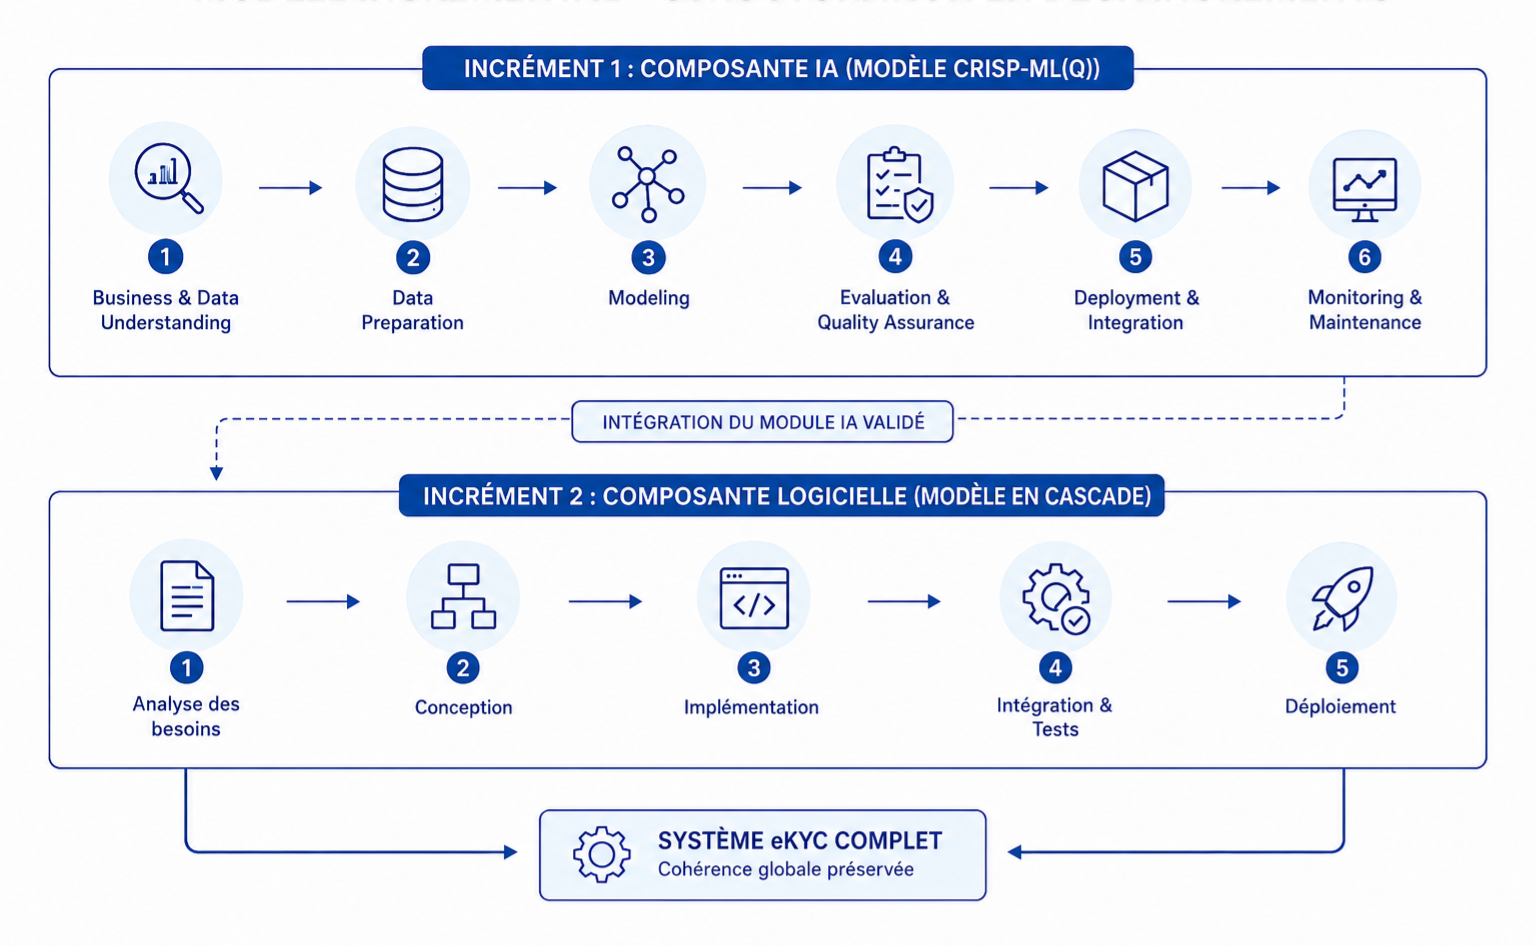
\includegraphics[width=\textwidth]{images/image_ch1/plannification du travail.PNG}
  \caption{\textit{Planification globale du projet selon l'approche incrémentale hybride}}
  \label{fig:ch1-planning}
\end{figure}

Cette structuration garantit que le module IA (composante la plus critique et la plus incertaine du projet) est pleinement validé avant d'être intégré à la plateforme applicative, réduisant ainsi les risques d'échec en phase d'intégration et assurant une livraison finale maîtrisée.


\section*{Conclusion du chapitre}

Ce chapitre a posé l'ensemble du cadre général du projet : présentation de la BTE et de sa plateforme NEO BTE, compréhension du métier KYC et de son cadre réglementaire, puis analyse critique des pratiques internes et des solutions commerciales disponibles. De ces analyses découle une problématique claire : l'incapacité du dispositif KYC actuel à assurer le passage à l'échelle qu'exige la stratégie digitale de la BTE, à laquelle répond une solution interne \textit{on-premise}, open-source et adaptée au contexte tunisien. La méthodologie hybride retenue garantit une structuration rigoureuse du développement en deux incréments complémentaires, dont les chapitres suivants détailleront les réalisations.
